\section{Objektliste}
\thispagestyle{fancy}

Grunna arbeidet rundt utforming av \gls{PID}, valde vi å lage ei liste over alle komponentane i anlegget som var tilkopla og styrt av styresystemet.
Objektlista inneheld tagg komponentbeskrivelse og plassering. 

I samband med innhenting av informasjon til dei ulike objekta har vi etablert ein database med datablad.
Databasen inneheld relevant informasjon om kvar enkelt komponent i styresystemet.\newline
Desse datablada er tilgjengeleg i vedlegg. (vedlegg I). 

I \gls{PLS}-programmet har vi nytta tagg for å namngi komponentane sine blokker.\newline
Objektlista gir høve til å knytte korrekt tagg til riktig komponent.

\newpage

\begin{tikzpicture}[remember picture, overlay]
    % Include the PDF page rotated, positioned at the center of the page
    \node[inner sep=0pt] at (current page.center) {
        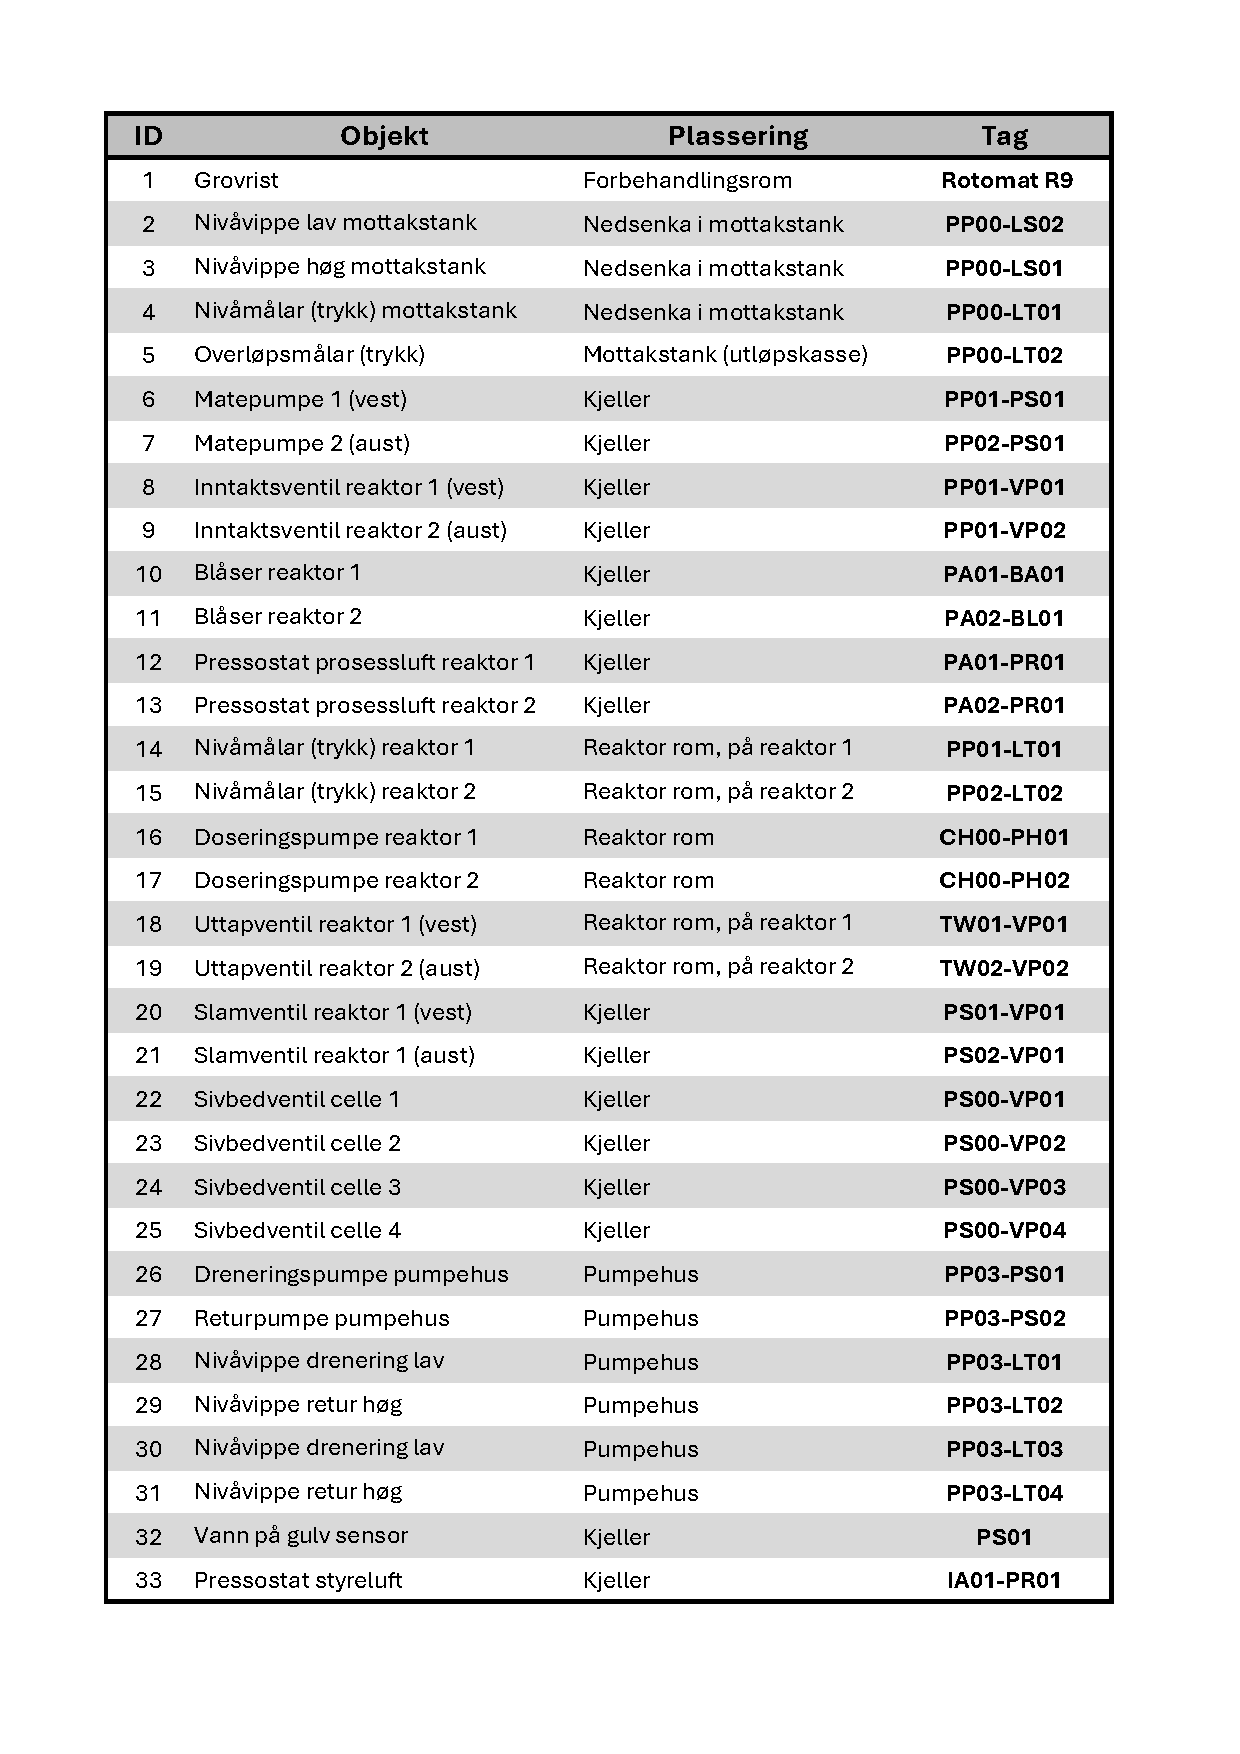
\includegraphics[page=1, scale=1, keepaspectratio]{Bilder/NyKomponentliste.pdf}
    };

    % Place the caption at the bottom of the page
    \node[anchor=south, yshift=10mm] at (current page.south) { % Adjust yshift to position the caption
        \begin{minipage}{\textwidth}
            \centering
            \captionof{figure}{Objektliste}
            \label{fig:SCD}
        \end{minipage}
    };
\end{tikzpicture}
